\chapter{Result}

\section{Methods Comparison Result}

For the methods in Chapter 2, we sorted genes according to the computed measure of the strength of evidence for DE, which were the adjusted p-values for alternative methods and the statistics shown in Equation \eqref{eq:10} for the \texttt{eBayes} method. From these sorted lists, we calculated area under ROC curve (AUC) values to evaluate the ability of these methods to distinguish genes with DE. 

To evaluate the true positive rate (TPR) and false positive rate (FPR) together, we generated receiver operator characteristic (ROC) curves based on the DE analysis results of the simulated datasets in each simulation scenario. It is a plot of the true positive rate against the false positive rate for the different possible cutpoints of a test (DE test). The slope of the tagent line at a cutpoint gives the likelihood ratio for that value of the test. Figure \ref{sc1_roc} is an example of the ROC curves we generated based on scenario 1 all simulated datasets. More scenario simulation ROC curves are in the Appendix. 

\begin{figure}[h!tb] 
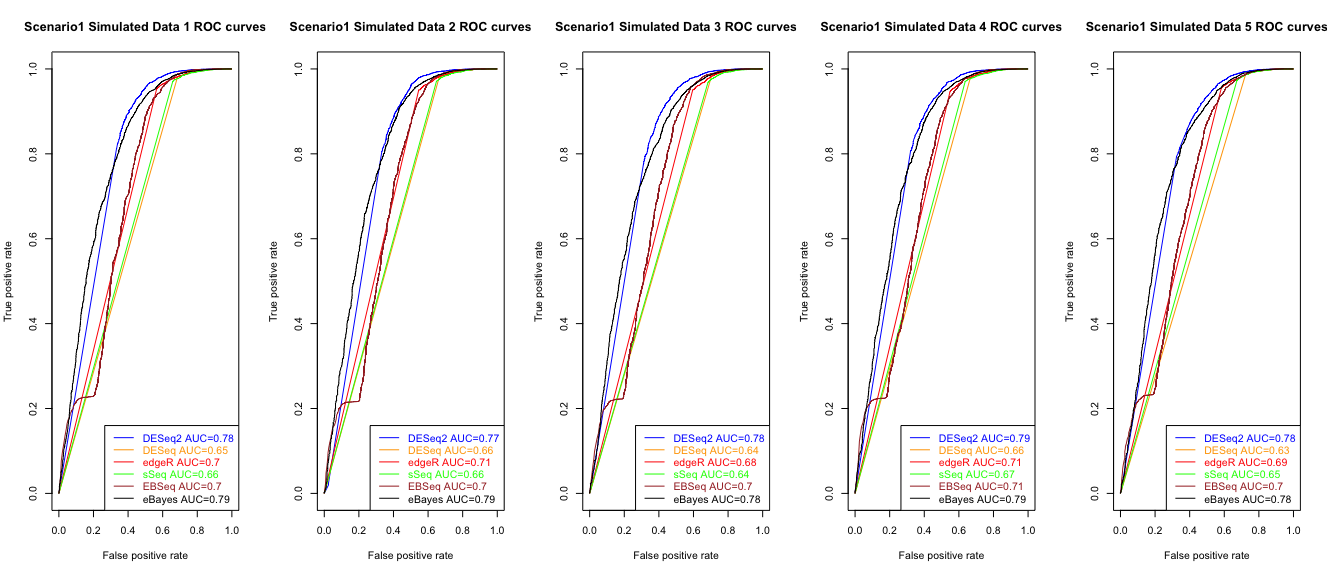
\includegraphics[height=6cm,width=15cm]{sc1_roc}
\caption{ROC curves of Simulated Datasets with $nGenes=10000, nSamples=8, pDiff=10\%$}
\label{sc1_roc}
\end{figure}


\begin{figure}[h!tb] 
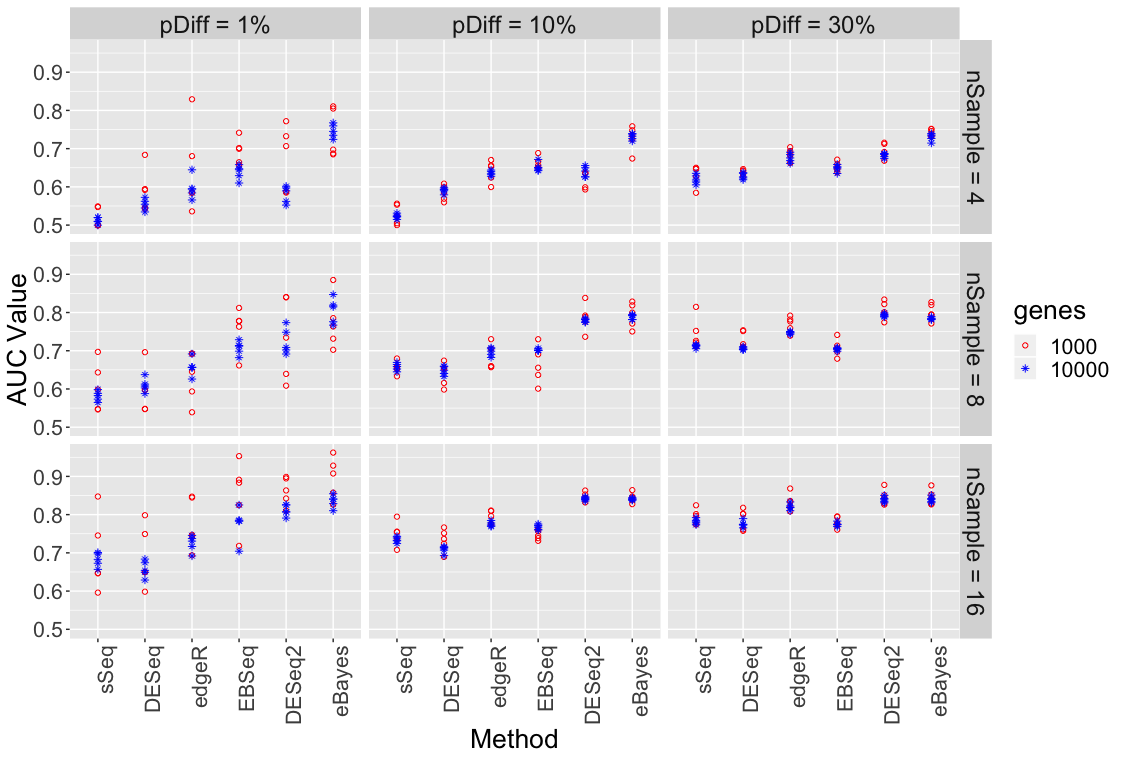
\includegraphics[height=10cm,width=15cm]{auc_plot}
\caption{AUC Plot of Simulated Datasets across Six Methods, Facetted by proportion of DE (pDiff) and number of samples (nSample), Grouped by total number of Genes (nGenes)}
\label{auc}
\end{figure}


We also evaluated the different methods with another performance metric: area under the curve (AUC) of ROC curves. The accuracy of the DE test depends on how well the test seperates the DE and non-DE groups. Accuracy is measured by the area under the ROC curve. Figure \ref{auc} provides the area under the ROC curve (AUC) across the 5 simulations for each of the scenario defined in \ref{tab:Scenario}. We facetted the plots by number of samples (nSample) and differential gene expression proportion (pDiff), grouped by different level of total number of genes. 

Similar to the single ROC curve, the \texttt{eBayes} method appears to outperform the other methods in terms of AUC, when number of samples and true DE proportion are small. With four or eight replicates per variety, there does not appear to be much of a difference between \texttt{eBayes} and {\tt DESeq2}, but as the number of replicates decreases, the \texttt{eBayes} approach appears to improve relative to {\tt DESeq2} in terms of AUC values.

We noticed that the difference among methods increased as proportion of true DE genes (pDiff) decreased. pDiff shrank means fewer genes were taged as true DE genes. \texttt{eBayes} seems a better DE genes analysis tool handling smaller pDiff. We also found that all methods perform better when the number of samples increases, while the number of genes (nGenes) doesn't affect the methods performance obviously in terms of AUC values. 







